\subsection{\Glsfmtfull{bert}}

\Gls{bert} est un \gls{llm} pré-entraîné de Google.
Il s'agit d'une \emph{pile d'encodeur de transformeur} (voir Figure~\ref{fig.bert}).
\gls{bert} existe en deux versions : 
\emph{base}, constitué de 12 couches d'encodeur et \emph{large}, constitué de 24. 
Ils ont respectivement 110M et 340M de paramètres~\cite{Devlin_Chang_Lee_Toutanova_2019}.

\begin{figure}[hbt]
    \centering
    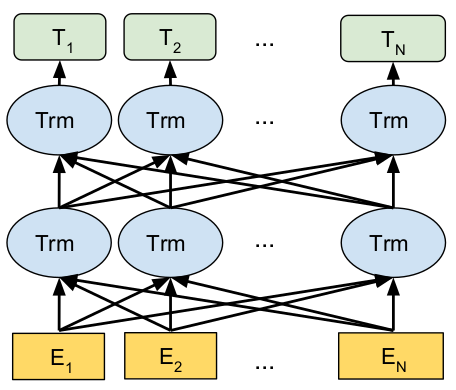
\includegraphics[width=.6\linewidth]{assets/images/bert.png}
    \caption[Architecture de \glsfmtshort{bert}.]%
    {Architecture de \glsfmtshort{bert}~\cite{Devlin_Chang_Lee_Toutanova_2019}}.
    \label{fig.bert}
\end{figure}

Tout comme \gls{gpt}, \gls{bert} est pré-entraîné d'une manière autosupervisée
puis affiné sur une tâche spécifique.
Pour le pré-entraînement de \gls{bert}, deux tâches sont utilisées.
La première est la \gls{mlm}.
Dans cette tâche, un pourcentage de tokens est aléatoirement remplacé par un token spécial \texttt{[MASK]}.
Le modèle doit alors prédire les tokens cachés en prenant le reste de la phrase comme contexte.
La deuxième tâche est la \gls{nsp}.
Pour cette tâche, deux phrases sont concaténées 
et le modèle doit prédire si la deuxième phrase est la suite de la première~\cite{Devlin_Chang_Lee_Toutanova_2019}.

À son tour, \gls{bert} a motivé l'apparition de plusieurs variantes.
En effet, il est l'un des modèles les plus réimplémentés dans la littérature à raison d'êtres open-source.
Parmi les variantes, on peut citer :
RoBERTa~\cite{Liu_Ott_Goyal_Du_Joshi_Chen_Levy_Lewis_Zettlemoyer_Stoyanov_2019},
qui est identique à \gls{bert} sauf qu'il utilise un processus de pré-entraînement différent,
CamemBERT~\cite{Martin_Muller_Ortiz_Suárez_Dupont_Romary_de_la_Clergerie_Seddah_Sagot_2020},
qui est une version française de \gls{bert}.

Plusieurs travaux dans la littérature ont utilisé \gls{bert}
pour la \gls{nmt}~\cite{Clinchant_Jung_Nikoulina_2019,Zhu_Xia_Wu_He_Qin_Zhou_Li_Liu_2020}.
Certains l'ont même utilisé pour la représentation des phrases aphasiques pour la classification%
~\cite{Qin_Lee_Kong_Lin_2022}.


